\documentclass[tikz,border=4pt]{standalone}
% Paleta y fuentes compartidas por el libro y las figuras (única fuente de verdad).
\RequirePackage{xcolor}
\definecolor{oxido}{HTML}{B7410E}
\definecolor{cobre}{HTML}{D27D2D}
\definecolor{carbon}{HTML}{2B2B2B}
\definecolor{azul}{HTML}{1F5F8B}
\definecolor{arena}{HTML}{F4EDE4}

\usepackage{fontspec}
\setsansfont{FiraSans}[Extension=.otf,UprightFont=*-Regular,BoldFont=*-SemiBold,ItalicFont=*-Italic,BoldItalicFont=*-SemiBoldItalic]
\setmonofont{FiraMono}[Extension=.otf,UprightFont=*-Regular,BoldFont=*-Medium,Scale=0.95]
\usetikzlibrary{positioning,arrows.meta,calc,decorations.pathreplacing}
\begin{document}
\sffamily\small
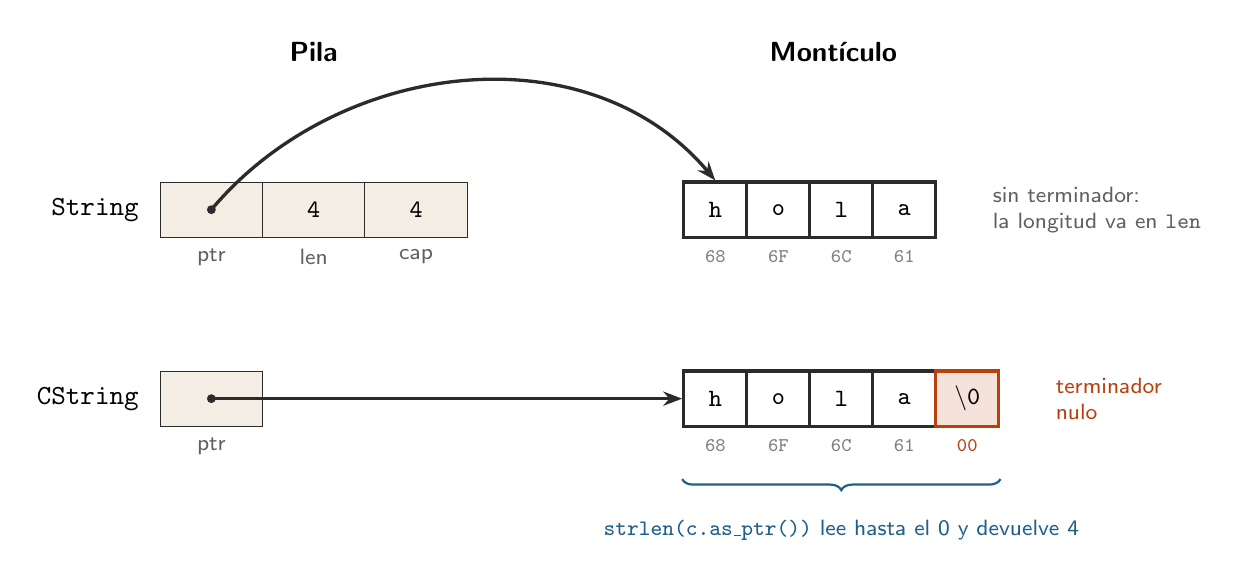
\begin{tikzpicture}[>={Stealth[length=2.4mm]},
  celda/.style={draw=carbon,minimum height=7mm,minimum width=13mm,font=\ttfamily\small},
  byte/.style={draw=carbon,very thick,minimum height=7mm,minimum width=8mm,font=\ttfamily\small,fill=white},
  rotulo/.style={font=\sffamily\footnotesize\color{carbon!75}},
  nota/.style={font=\sffamily\footnotesize,text=carbon!75,anchor=west,align=left}]
  % Encabezados
  \node[font=\sffamily\bfseries] at (1.3,2.0) {Pila};
  \node[font=\sffamily\bfseries] at (7.9,2.0) {Montículo};
  % ---- String ----
  \node[anchor=east,font=\ttfamily\bfseries] at (-0.8,0) {String};
  \foreach \c/\v [count=\i from 0] in {ptr/{}, len/4, cap/4} {
    \node[celda,fill=arena] (s\i) at (\i*1.3,0) {\v};
    \node[rotulo] at (\i*1.3,-0.6) {\c};
  }
  \foreach \l/\h [count=\i from 0] in {h/68,o/6F,l/6C,a/61} {
    \node[byte] (a\i) at (6.4+\i*0.8,0) {\l};
    \node[rotulo,font=\ttfamily\scriptsize\color{carbon!60}] at (6.4+\i*0.8,-0.6) {\h};
  }
  \fill[carbon] (s0.center) circle (1.6pt);
  \draw[->,very thick,carbon] (s0.center) to[out=50,in=130] (a0.north);
  \node[nota] at (9.8,0) {sin terminador:\\la longitud va en \texttt{len}};
  % ---- CString ----
  \node[anchor=east,font=\ttfamily\bfseries] at (-0.8,-2.4) {CString};
  \node[celda,fill=arena] (c0) at (0,-2.4) {};
  \node[rotulo] at (0,-3.0) {ptr};
  \foreach \l/\h [count=\i from 0] in {h/68,o/6F,l/6C,a/61} {
    \node[byte] (b\i) at (6.4+\i*0.8,-2.4) {\l};
    \node[rotulo,font=\ttfamily\scriptsize\color{carbon!60}] at (6.4+\i*0.8,-3.0) {\h};
  }
  \node[byte,fill=oxido!15,draw=oxido] (b4) at (6.4+4*0.8,-2.4) {\textbackslash 0};
  \node[rotulo,font=\ttfamily\scriptsize\color{oxido}] at (6.4+4*0.8,-3.0) {00};
  \fill[carbon] (c0.center) circle (1.6pt);
  \draw[->,very thick,carbon] (c0.center) -- (b0.west);
  \node[nota,text=oxido] at (10.6,-2.4) {terminador\\nulo};
  % ---- Lado de C ----
  \draw[decorate,decoration={brace,amplitude=4pt,mirror},azul,line width=0.8pt]
    ($(b0.south west)+(0,-0.65)$) -- ($(b4.south east)+(0,-0.65)$);
  \node[font=\sffamily\footnotesize,text=azul,anchor=north] at ($(b2.south)+(0,-1.05)$)
    {\texttt{strlen(c.as\_ptr())} lee hasta el 0 y devuelve 4};
\end{tikzpicture}
\end{document}
